\documentclass[10pt,a4paper]{article}
\usepackage[utf8]{inputenc}
\usepackage[spanish]{babel}
\usepackage{amsmath}
\usepackage{amsfonts}
\usepackage{amssymb}
\usepackage{enumitem}
\usepackage{hyperref} 
\usepackage{graphicx}
\usepackage[table]{xcolor}
\hypersetup{pdftex,colorlinks=true,allcolors=blue}
\hypersetup{
    pdftitle={},
    pdfauthor={Pablo Riutort Grande},
    pdfsubject={},
    bookmarksnumbered=true,     
    bookmarksopen=true,         
    bookmarksopenlevel=1,       
    colorlinks=true,            
    pdfstartview=Fit,           
    pdfpagemode=UseOutlines,    % this is the option you were lookin for
    pdfpagelayout=TwoPageRight
}
\usepackage{listings}
\usepackage{xcolor}
\usepackage{hypcap}
\definecolor{codegreen}{rgb}{0,0.6,0}
\definecolor{codegray}{rgb}{0.5,0.5,0.5}
\definecolor{codepurple}{rgb}{0.58,0,0.82}
\definecolor{backcolour}{rgb}{0.95,0.95,0.92}
\lstdefinestyle{mystyle}{
    backgroundcolor=\color{backcolour},   
    commentstyle=\color{codegreen},
    keywordstyle=\color{magenta},
    numberstyle=\tiny\color{codegray},
    stringstyle=\color{codepurple},
    basicstyle=\ttfamily\footnotesize,
    breakatwhitespace=false,         
    breaklines=true,                 
    captionpos=b,                    
    keepspaces=true,                 
    numbers=left,                    
    numbersep=5pt,                  
    showspaces=false,                
    showstringspaces=false,
    showtabs=false,                  
    tabsize=2
}

\lstset{style=mystyle}
\usepackage{xparse}
\NewDocumentCommand{\codeword}{v}{%
\texttt{{#1}}
}
\author{Pablo Riutort Grande}
\title{PEC 1\\ \vspace{1cm}\textbf{Descripción de los sistemas Biométricos y su evaluación}}
\begin{document}
\maketitle
\pagebreak

\section{}
\subsection{}

\begin{itemize}
\item \textbf{Universalidad:}
Una gran mayoría de la población contiene ambos rasgos salvo contadas excepciones. En el caso de las venas, dependiendo de la extermidad para que el lector esté diseñado puede que haya personas que no puedan utilizarlo.
\item \textbf{Particularidad:} Las venas presentan una distribución geométrica única para cada persona \cite{venas}, por tanto, es un rasgo muy particular. La voz, aunque también es única para cada individuo \cite{voz}, puede ser imitada por otra persona.
\item \textbf{Permanencia} Las venas son invariables a lo largo del tiempo, salvo casos excepcionales \cite{venas}, por otra parte, la voz, puede sufrir grandes cambios en según qué edades de la persona y en según qué estado se encuentre.
\item \textbf{Medible} Tanto en la voz como en las venas vemos que existen distintos dispositivos diseñados específicamente para medir los rasgos; micrófonos y cámaras de infrarrojos.
\item \textbf{Aceptabilidad} Los estudios demuestran que la gente está dispuesta a identificarse por voz \cite{voz} y por lo general con biometría.
\item \textbf{No falsificable} La voz puede ser falsificable bien por otra persona o grabada y reproducida mediante un dispositivo. En cuanto a las venas, puesto que el patrón es único, es difícilmente falsificable.
\end{itemize}

\begin{table}[htpb!]
\resizebox{\textwidth}{!}{
\begin{tabular}{|c|c|c|c|c|c|c|c|}
\hline
\textbf{Rasgo biométrico} & \textbf{Universalidad} & \textbf{Particularidad} & \textbf{Permanencia} & \textbf{Medible} & \textbf{Aceptabilidad}  & \textbf{No falsificable} \\ \hline
\textbf{Venas} & A & A & A & M & M & A \\ \hline
\textbf{Voz} & A & B & B & M & A & B \\ \hline
\end{tabular}
}
  \caption{Bondad de los rasgos biométricos vasculares y de voz discretizada en tres valores: A (alto), M (medio) y B (bajo)}
  \label{tabla:bondad1}
\end{table}

\subsection{}
\begin{table}[htpb!]
\resizebox{\textwidth}{!}{
\begin{tabular}{|c|c|c|c|c|c|c|c|}
\hline
\textbf{Rasgo biométrico} & \textbf{Universalidad} & \textbf{Particularidad} & \textbf{Permanencia} & \textbf{Medible}  & \textbf{Rendimiento} & \textbf{Aceptabilidad}  & \textbf{No falsificable} \\ \hline
\textbf{Venas} & M & M & M & M & M & M & A \\ \hline
\textbf{Voz} & M & B & B & M & B & A & B \\ \hline
\end{tabular}
}
  \caption{Bondad de los rasgos biométricos vasculares y de voz \cite{handbook}}
  \label{tabla:bondad2}
\end{table}
Los requisitos donde hay discrepancia son en universalidad, particularidad y permanencia.\\
En cuanto al rasgo de universiladidad, quizá se haya considerado a las personas que no sean hablantes o que no posean manos que poder ser analizadas por un lector pero, dado que estos casos son muy raros, considero que la universalidad es alta.\\
En la particularidad y permanencia de las venas, discrepo completamente, puesto que el patrón de venas que presentamos es único para cada persona a lo largo del tiempo. Quizá se necesite estudiar más la casuística de circunstancias médicas excepcionales o cómo afecta la edad a ese patrón, pero, en general son particulares y permanentes.

\section{}
\subsection{}
\begin{table}[htbp]
\resizebox{\textwidth}{!}{
\begin{tabular}{|c|c|c|c||c|c|c||c|c|c||c|c|c|}
\hline
 & \textbf{1\_1} & \textbf{1\_2}  & \textbf{1\_3}  & 
 \textbf{2\_1}  & \textbf{2\_2}  & \textbf{2\_3}  & 
 \textbf{3\_1}  & \textbf{3\_2}  & \textbf{3\_3}  & 
 \textbf{4\_1}  & \textbf{4\_2}  & \textbf{4\_3} \\ 
 \hline
 
  \textbf{1\_4} & \cellcolor{gray!25} 347 & \cellcolor{gray!25} 301 & \cellcolor{gray!25} 359 & 5 & 305 & 334 & 3 & 4 & 290 & 2 & 3 & 3 \\ \hline
  
  \textbf{2\_4} & 344 & 274 & 308 & \cellcolor{gray!25} 7 & \cellcolor{gray!25} 275 & \cellcolor{gray!25} 335 & 5 & 7 & 326 & 3 & 6 & 3 \\ \hline
  
  \textbf{3\_4} & 4 & 9 & 3 & 270 & 6 & 3 & \cellcolor{gray!25}254 & \cellcolor{gray!25}292 & \cellcolor{gray!25}9 & 268 &   194 & 283 \\ \hline
  
  \textbf{4\_4} & 3 & 8 & 3 & 264 & 8 & 3 & 318 & 341 & 9 & \cellcolor{gray!25}325 & \cellcolor{gray!25}297 & \cellcolor{gray!25}322 \\ \hline

\end{tabular}
}
  \caption{Medidas de similitud}
  \label{tabla:medidas}
\end{table}

Los intentos de identificación genuinos son aquellos marcados en negrita.\\
Como podemos observar, existen cierta similitud entre la identificación genuina de la persona 1 con la identificación de la persona 2, es decir, los valores obtenidos para el intento de identificación de la persona 2 como persona 1 son muy similares. Ocurre lo mismo con la persona 3 y el intento genuino de la persona 4 y viceversa.\\
Esto puede derivar en falsos positivos en función del umbral que se escoja, es decir, que el sistema de por buena la identificación de una persona cuando realmente no es quien dice ser.

\subsection{}
Dado un umbral, con que una de las tres comparaciones esté por encima de este entonces ya consideramos que tenemos una petición correcta. Dado que una columna se compone de 3 celdas y que estas después de comparar con el umbral se convierten en una, tendremos una nueva tabla formada por $n/3$ columnas, en nuestro caso $12/3 = 4$. \\
El umbral es 300, por tanto, cualquier conjunto que tenga al menos uno de sus 3 valores por encima de 300 se considera una identifiación correcta.
\begin{table}[h!]
\begin{center}

\begin{tabular}{|l|c|c|c|c|}
\hline
 & \textbf{1} & \textbf{2} & \textbf{3} & \textbf{4} \\ \hline
 
  \textbf{1} & 1 & 1 & 0 & 0 \\ \hline  
  \textbf{2} & 1 & 1 & 1 & 0 \\ \hline
  \textbf{3} & 0 & 0 & 0 & 0\\ \hline
  \textbf{4} & 0 & 0 & 1 & 1\\ \hline

\end{tabular}

  \caption{Matriz de similitud}
  \label{tabla:similitudes}
\end{center}
\end{table}

\pagebreak
\subsection{}
\begin{table}[h!]
\resizebox{\textwidth}{!}{
\begin{tabular}{|l|c|c|c|c|}
\hline
 & \textbf{1} & \textbf{2} & \textbf{3} & \textbf{4} \\ \hline
 
  \textbf{1} & AC: aceptación correcta & FA: falsa aceptación & RC: rechazo correcto & RC: rechazo correcto\\ \hline
  \textbf{2} & FA: falsa aceptación & AC: aceptación correcta & FA: falsa aceptación & RC: rechazo correcto\\ \hline
  \textbf{3} & RC: rechazo correcto & RC: rechazo correcto & FR: falso rechazo & RC: rechazo correcto\\ \hline
  \textbf{4} & RC: rechazo correcto & RC: rechazo correcto & FA: falsa aceptación & AC: aceptación correcta \\ \hline

\end{tabular}
}
  \caption{Comparaciones correctas o falsas}
  \label{tabla:comparaciones}
\end{table}

\subsubsection{}
La huella 03\_4.tif siempre es rechazada.
\subsubsection{}
Tanto las huellas 01\_4.tif como 02\_4.tif son aceptadas en las personas 1 y 2, además, la huella 02\_4.tif es también aceptada en la persona 3. La huella 04\_4.tif es aceptada en las persona 3 y 4.

\subsubsection{}
Ninguna huella del conjunto ha dado los cuatro resultados correctos.


\subsection{}
La razón de error de etiquetado (FMR) se calcula como el número de falsas aceptaciones dividido por la población impostora.

\begin{center}
$FMR = 4/12 = 1/4$

\end{center}
La razón de error de no etiquetado (FNMR) se calcula como el número de falsos
rechazos dividido por la población genuina.

\begin{center}
$FNMR = 1/4$
\end{center}

Para los valores del umbral (t) [Cuadro \ref{tabla:errors1}] obtenemos la siguiente gráfica:

\begin{figure}[h!]
  \centering
  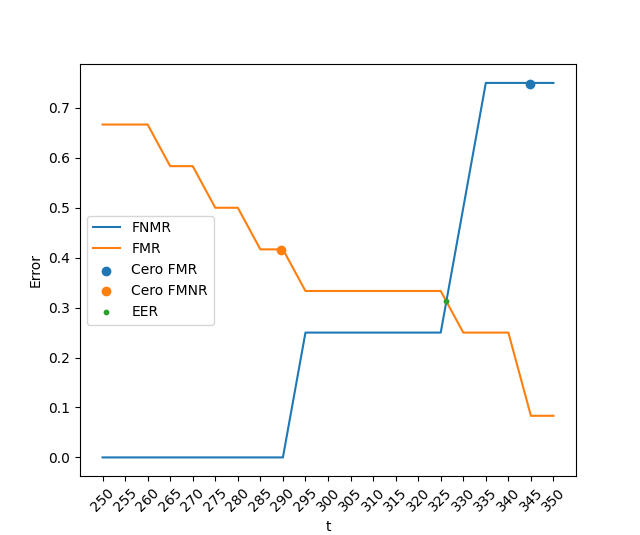
\includegraphics[scale=0.7]{errorsv1.png}\\
  \caption{Evolución de errores}
  \label{fig:errors2}
\end{figure}

\pagebreak

\subsection{}
El valor de EER indica la razón de error para todos los valores del umbral donde la FMR es igual a la FNMR, en nuestra gráfica podemos aproximar dicho valor a 0.31.\\
Cero FNMR se define como el valor menor de la FMR en el que no hay errores de etiquetado, en nuestro caso es 0.41.\\
Cero FMR se define como el valor menor de la FNMR en el que no hay errores de no etiquetado, en nuestra gráfica vemos que corresponde a 0.75.\\

Después de ver los resultados con el umbral proporcionado, quizá habría que aumentarlo para reducir la FMR a un valor cercano a la EER, entre 320 y 325.

\subsection{}
En una aplicación donde lo importante es que no entren intrusos, lo que nos preocupa es que la FMR sea alta, por tanto, habrá que poner un umbral de similitud mayor para hacer la aplicación más segura y bajando así la FMR. Un umbral próximo al cero FMR podría funcionar (335, 340). Las consecuencias de este umbral implicará que algunas veces personas autorizadas serán rechazadas por el sistema porque habrá aumentado la FNMR.\\
En caso contrario, en el que queremos que un usuario casi siempre sea identificado nos preocupa que la FNMR sea alta, por tanto, habrá que desplazar el umbral de similitud en sentido opuesto, cerca del cero FNMR (285, 290), implicando así, a su vez, que la FMR aumente.

\subsection{}
El valor 1 - FNMR(t) se denomina la bondad del test. Si queremos que la bondad sea de 0.5:\\

\begin{center}
1 - FNMR(t) = 0.5 \\
FNMR(t) = 0.5 
\end{center}

El valor de t donde FNMR = 0.5 es 330 [Cuadro \ref{tabla:errors1}].\\



\begin{table}[h!]
\begin{center}
\begin{tabular}{|c|c|c|}
\hline
\textbf{umbral (\textit{t})} & \textbf{FMR} & \textbf{FNMR}  \\ \hline
250 & 0.6666666666666666 & 0.0 \\ \hline
255 & 0.6666666666666666 & 0.0 \\ \hline
260 & 0.6666666666666666 & 0.0 \\ \hline
265 & 0.5833333333333334 & 0.0 \\ \hline
270 & 0.5833333333333334 & 0.0 \\ \hline
275 & 0.5 & 0.0 \\ \hline
280 & 0.5 & 0.0 \\ \hline
285 & 0.4166666666666667 & 0.0 \\ \hline
290 & 0.4166666666666667 & 0.0 \\ \hline
295 & 0.3333333333333333 & 0.25 \\ \hline
300 & 0.3333333333333333 & 0.25 \\ \hline
305 & 0.3333333333333333 & 0.25 \\ \hline
310 & 0.3333333333333333 & 0.25 \\ \hline
315 & 0.3333333333333333 & 0.25 \\ \hline
320 & 0.3333333333333333 & 0.25 \\ \hline
325 & 0.3333333333333333 & 0.25 \\ \hline
330 & 0.25 & 0.5 \\ \hline
335 & 0.25 & 0.75 \\ \hline
340 & 0.25 & 0.75 \\ \hline
345 & 0.08333333333333333 & 0.75 \\ \hline
350 & 0.08333333333333333 & 0.75 \\ \hline
\end{tabular}
\end{center}
  \caption{valores del umbral (t)}
  \label{tabla:errors1}

\end{table}

\pagebreak

\begin{thebibliography}{9}

\bibitem{handbook}
	\textbf{''Handbook of Fingerprint Recognition''}, \\
	\textit{Davide Maltoni, Dario Maio, Anil K. Jain, Salil Prabhakar.} \\
	Springer Publishing Company, 2009, ISBN: 1848822537
  
\bibitem{biometria}
  \textbf{''La biometría parala identificación de las personas''}, \\
  \textit{Francesc Serratosa.}\\
  UOC, Cap. 4. Los rasgos biométricos. Pag 22
  
\bibitem{venas}
  \textbf{''Venas de las manos''}, \\
  EcuRed.\\
  \href{https://www.ecured.cu/Venas_de_las_manos}{www.ecured.cu/Venas\_de\_las\_manos}
  
\bibitem{voz}
  \textbf{''Autenticación biométrica: ¿pueden «robarme» la voz?''}, \\
  Bit Life Media.\\
  \href{https://bitlifemedia.com/2018/09/autenticacion-biometrica-pueden-robarme-la-voz/}{bitlifemedia.com/2018/09/autenticacion-biometrica-pueden-robarme-la-voz/}

\end{thebibliography}

\pagebreak

\appendix
\section{Código auxiliar}
\label{appendix:help}
A continuación se expone el programa utilizado para la generación de la tabla de comparaciones [Cuadro \ref{tabla:comparaciones}],  los valores FMR y FNMR para ciertos umbrales [Cuadro \ref{tabla:errors1}] y su respectiva gráfica [Fig. \ref{fig:errors2}] a partir de las medidas de similitud [Cuadro \ref{tabla:medidas}].
\lstinputlisting[language=Python]{v2.py}




\end{document}